% !TEX root = ../reporte_final.tex
\section{Diseño y ejecución de los experimentos}

\subsection{Exploración de datos}

El dataset cargado contiene 344 observaciones y 8 columnas (4 numéricas, 4 categóricas). La distribución por especie es desbalanceada: \emph{Adelie} con 152 ejemplares, \emph{Gentoo} con 124 y \emph{Chinstrap} con 68. Tras eliminar las filas con valores faltantes en cualquiera de las cuatro variables numéricas o en \texttt{species}, el dataset definitivo queda en 342 filas (\emph{Adelie}: 151, \emph{Gentoo}: 123, \emph{Chinstrap}: 68).

\begin{figure}[H]
\centering
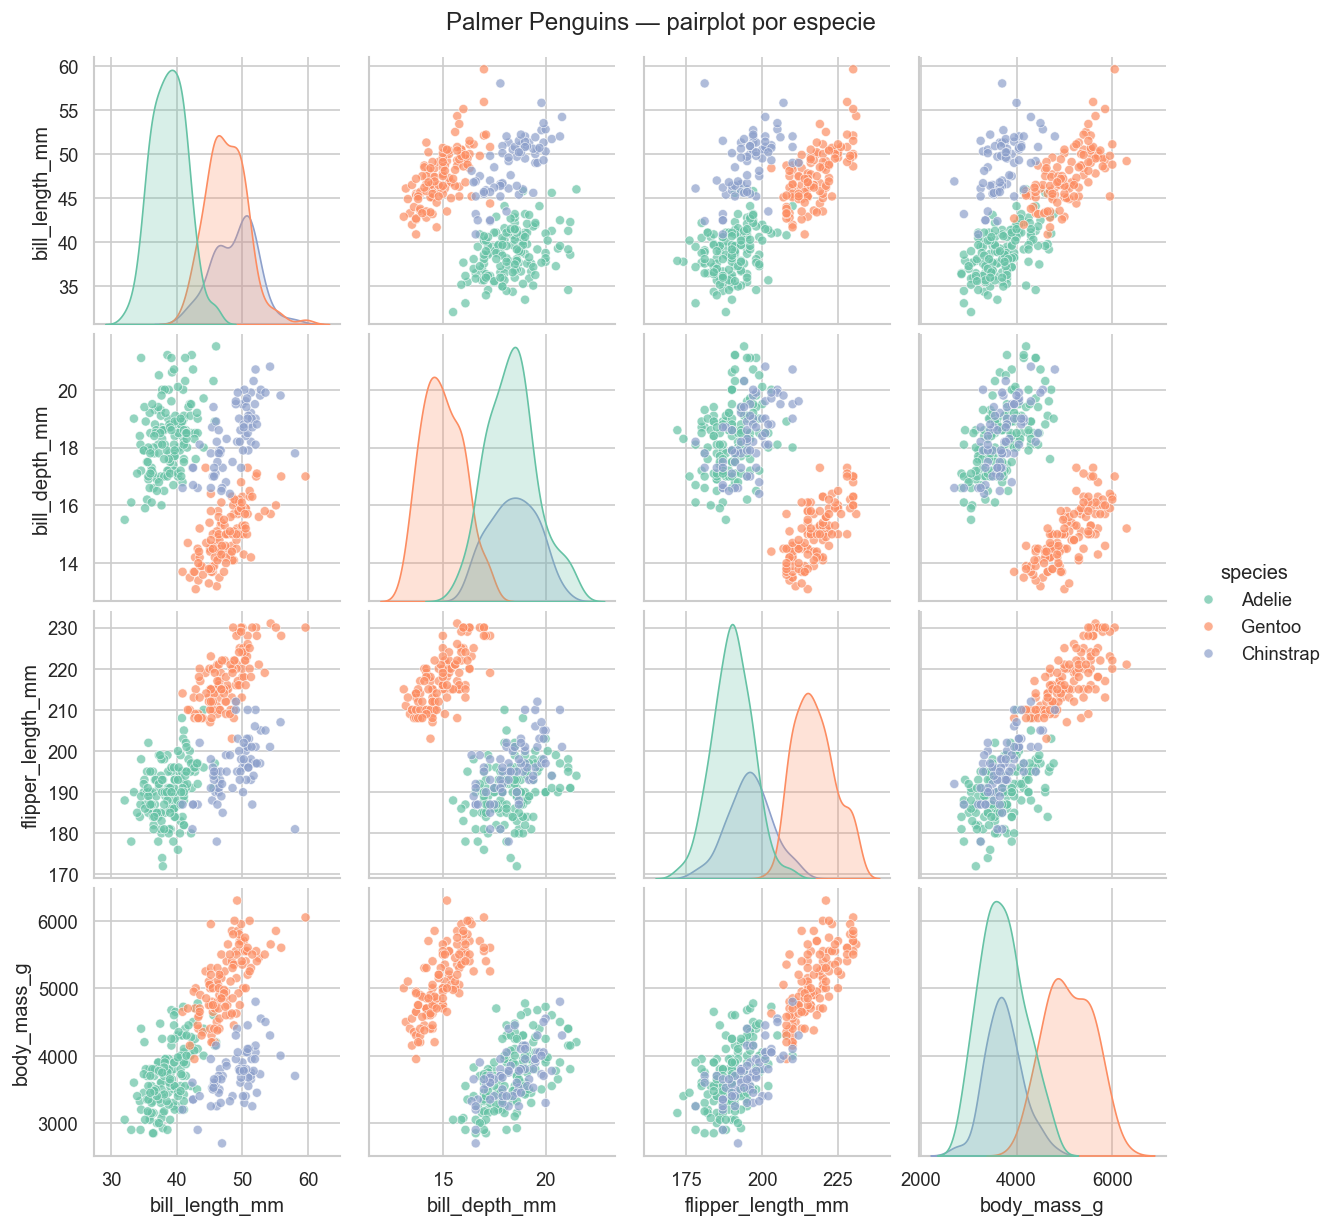
\includegraphics[width=0.98\linewidth]{images/pairplot.png}
\caption{\emph{Pairplot} de las cuatro variables morfométricas discriminado por especie. \emph{Gentoo} se separa claramente del par \emph{Adelie}/\emph{Chinstrap}, especialmente en \texttt{flipper\_length\_mm} y \texttt{body\_mass\_g}. \emph{Adelie} y \emph{Chinstrap} comparten masa corporal y longitud de aleta similares, pero se distinguen por la longitud del pico.}
\label{fig:pairplot}
\end{figure}

\begin{figure}[H]
\centering
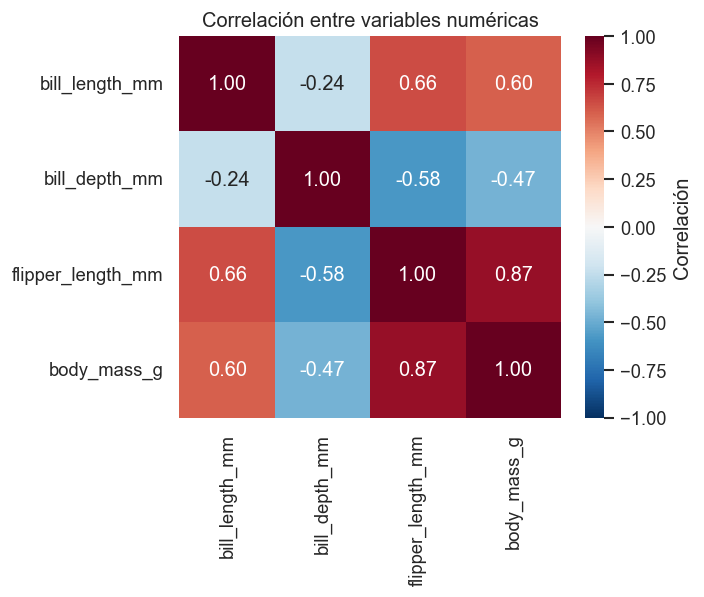
\includegraphics[width=0.62\linewidth]{images/correlacion.png}
\caption{Matriz de correlación de Pearson entre las variables numéricas. La correlación más fuerte se da entre \texttt{flipper\_length\_mm} y \texttt{body\_mass\_g} ($\rho \approx 0.87$). La correlación negativa de $-0.58$ entre \texttt{bill\_depth\_mm} y \texttt{flipper\_length\_mm} es una manifestación de la paradoja de Simpson causada por la mezcla de especies.}
\label{fig:corr}
\end{figure}

\subsection{Determinación del número de clusters}

Antes de fijar $k=3$ se aplicó el \emph{método del codo} para K-Means barriendo $k\in\{1,\dots,8\}$. La figura~\ref{fig:codo} muestra la inercia decreciente con un quiebre visible en $k=3$, congruente con la presencia de tres especies en el dataset.

\begin{figure}[H]
\centering
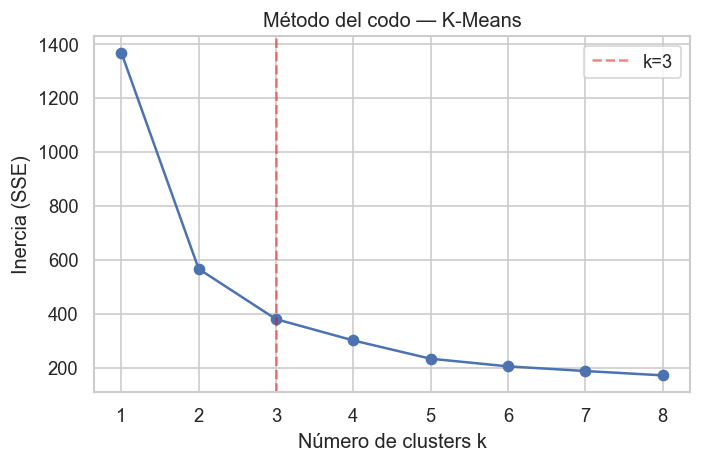
\includegraphics[width=0.62\linewidth]{images/codo.png}
\caption{Método del codo para K-Means sobre las variables estandarizadas. El descenso de la inercia presenta un quiebre en $k=3$.}
\label{fig:codo}
\end{figure}

\subsection{Configuración de los algoritmos}

La tabla~\ref{tab:hyper} consigna los hiperparámetros utilizados; todos los demás se dejan en los valores por omisión de \texttt{scikit-learn}. La semilla \texttt{RANDOM\_STATE} = 42 aplica a K-Means; DBSCAN y Agglomerative son deterministas.

\begin{table}[H]
\centering
\caption{Hiperparámetros de los algoritmos comparados.}
\label{tab:hyper}
\begin{tabularx}{\textwidth}{l >{\hsize=0.85\hsize\raggedright\arraybackslash}X >{\hsize=1.15\hsize\raggedright\arraybackslash}X}
\toprule
\textbf{Algoritmo} & \textbf{Hiperparámetros} & \textbf{Justificación}\\
\midrule
K-Means       & \texttt{n\_clusters=3}, \texttt{n\_init=10}                & $k=3$ por método del codo y por la verdad biológica.\\
DBSCAN        & \texttt{eps=0.6}, \texttt{min\_samples=5}                  & Valor por defecto típico tras estandarización; sin búsqueda fina.\\
Agglomerative & \texttt{n\_clusters=3}, \texttt{linkage="ward"}            & Ward favorece clusters compactos y de varianza homogénea.\\
\bottomrule
\end{tabularx}
\end{table}
